\chapter{Deep Learning for Image Classification}

\section{Convolutional Neural Networks}
Convolutional Neural Networks (CNN) are the most widespread architecture
for image processing in DL. They are based on the idea of convolutional
filters, which are small matrices that slide over the input image to
detect local patterns. The main advantage of CNNs is their ability to
learn hierarchical representations of the data, where lower layers
detect simple features (e.g., edges, textures) and higher layers
detect more complex features (e.g., shapes, objects). This hierarchical
representation allows CNNs to achieve state-of-the-art performance in
various image classification tasks, such as object detection,
semantic segmentation, and image generation.

\begin{figure}[htbp]
   \centering
   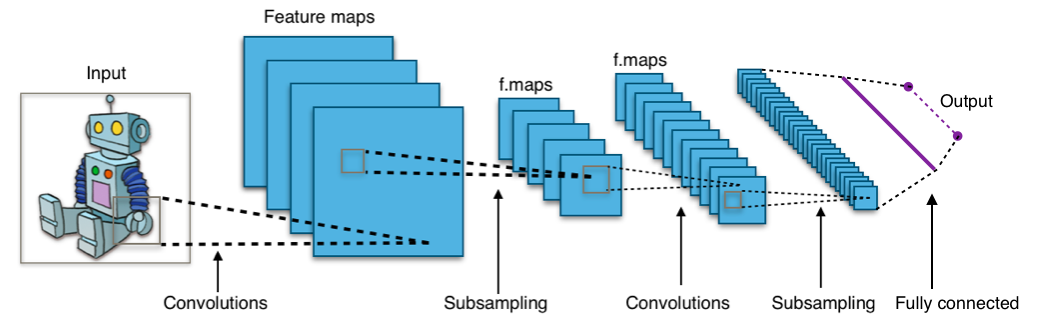
\includegraphics{images/10/cnn.png}
   \caption{Typical CNN architecture}
   \label{fig:10/cnn}
\end{figure}

Main components:
\begin{itemize}
	\item Convolutional blocks: convolutions, activation functions, subsampling
	\item Classification/regression block: fully connected layers
\end{itemize}
Trainable componentes:
\begin{itemize}
	\item Convolution values
	\item Fully connected layers weights
\end{itemize}

\begin{paracol}{2}
   
   The process is based on 2D convolution.
   In each convolution block we have the following features:
   \begin{itemize}
      \item \textbf{Kernel size} $K$: usually small kernels ($3\times 3, 5\times 5, \dots$ )
      \item \textbf{Number of filters} $F$: how many different kernels are used
      \item \textbf{Padding size} $P$: border padding, usually with zero values
      \item \textbf{Stride} $S$: pixel sampling, $S = 1$ means all pixels
   \end{itemize}

   \switchcolumn

   \begin{figure}[htbp]
      \centering
      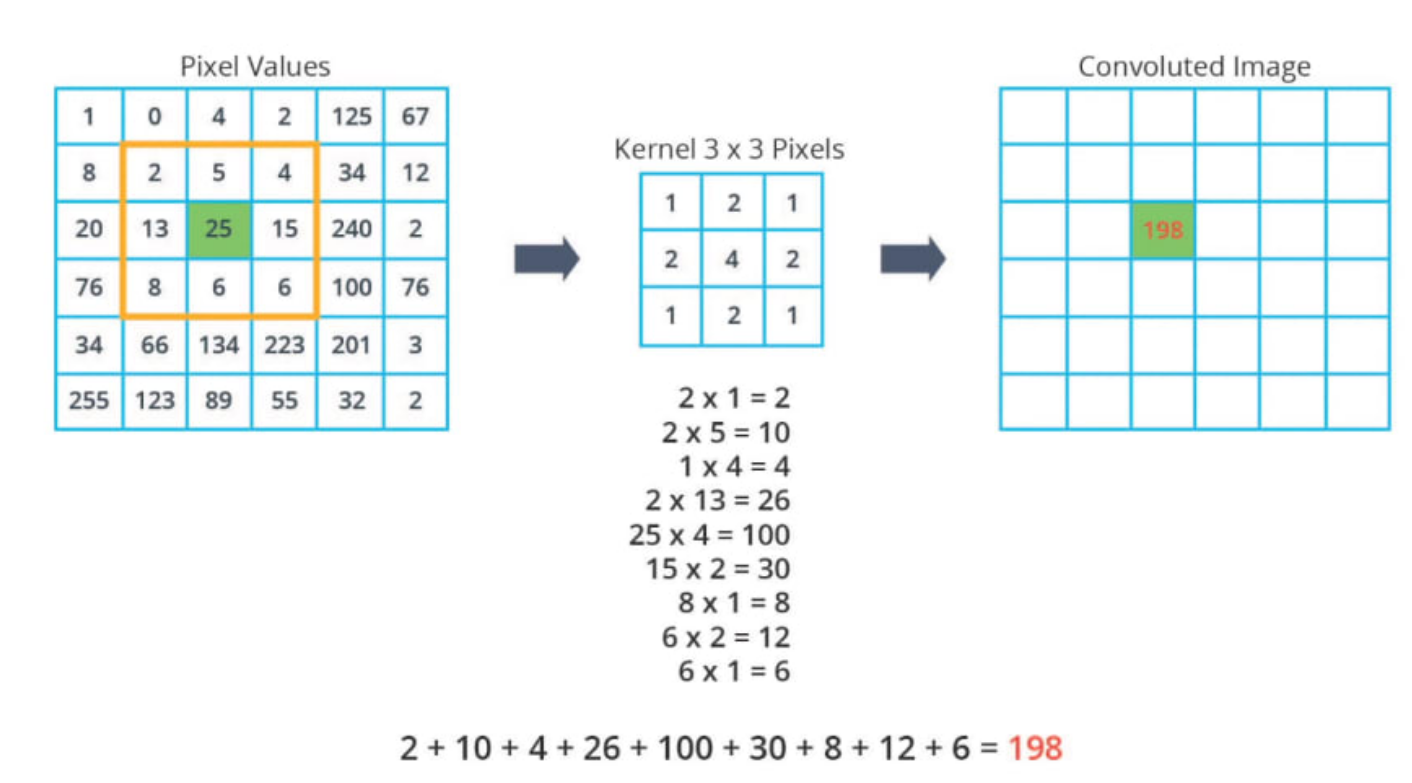
\includegraphics{images/10/convolution2d.png}
      \caption{Example of 2D convolution}
      \label{fig:10/convolution2d}
   \end{figure}
\end{paracol}

Each convolutional block has as output a set of $F$ maps; 
each map is built by the application of the corresponding filter to each possible pixel/component of the input.
\nl

Size for each map is the following (for $H\times W$ input):
\[\frac{1}{S^2} (H + 2P - (K - 1))(W + 2P - (K-1))\]
Spatial cost mainly dependent on number of filters.
\nl

The total number of products (for $H\times W$ input) instead: 
\[K^2\frac{F}{S^2} (H + 2P - (K - 1))(W + 2P - (K-1))\]
Temporal cost mainly dependent on kernel size

\subsection{Pooling}

Usual activation function: $ReLU$
% // TODO

Subsampling (pooling):
\begin{itemize}
	\item Allows generalization and improves robustness
	\item Reduces size and computational cost
	\item Fixed operators, small square size ($2\times 2$)
\end{itemize}

Subsampling is usually done after each convolutional block, and consists of reducing the spatial dimensions of feature maps while preserving their important information. The most common types of pooling are:

\begin{figure}[htbp]
   \centering
   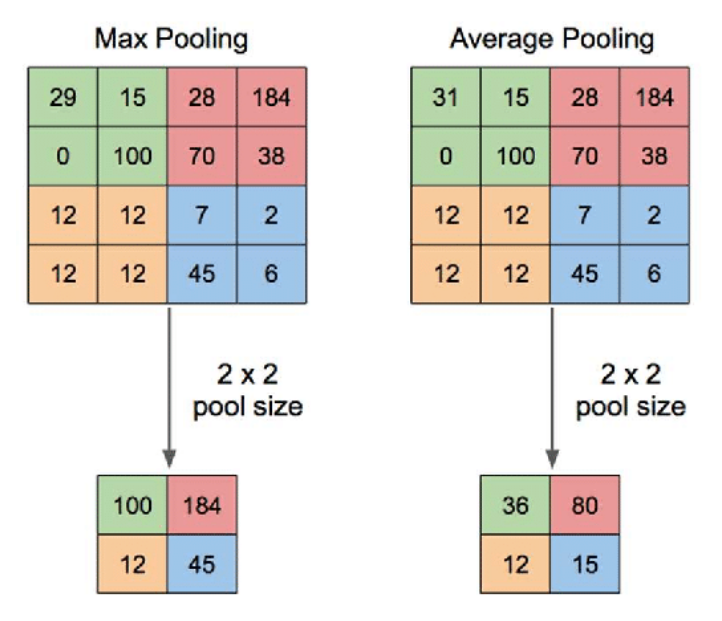
\includegraphics{images/10/pooling.png}
   \caption{Different types of pooling operations}
   \label{fig:10/pooling}
\end{figure}

\begin{itemize}
   \item \textbf{Max pooling}: Takes the maximum value in each window
   \item \textbf{Average pooling}: Takes the average of all values in the window
   \item \textbf{Global pooling}: Applies pooling across the entire feature map
\end{itemize}

Max pooling is most commonly used because it helps in:
\begin{itemize}
   \item Retaining the strongest features
   \item Making the network more invariant to small translations
   \item Reducing spatial dimensions, which decreases computation
   \item Controlling overfitting by reducing the number of parameters
\end{itemize}

The output size after applying pooling with window size $P$ and stride $S$ is:
\[\lfloor\frac{W - P}{S} + 1\rfloor \times \lfloor\frac{H - P}{S} + 1\rfloor\]
% //TODO verify

\subsubsection{Convolutional Blocks}
\begin{figure}[htbp]
   \centering
   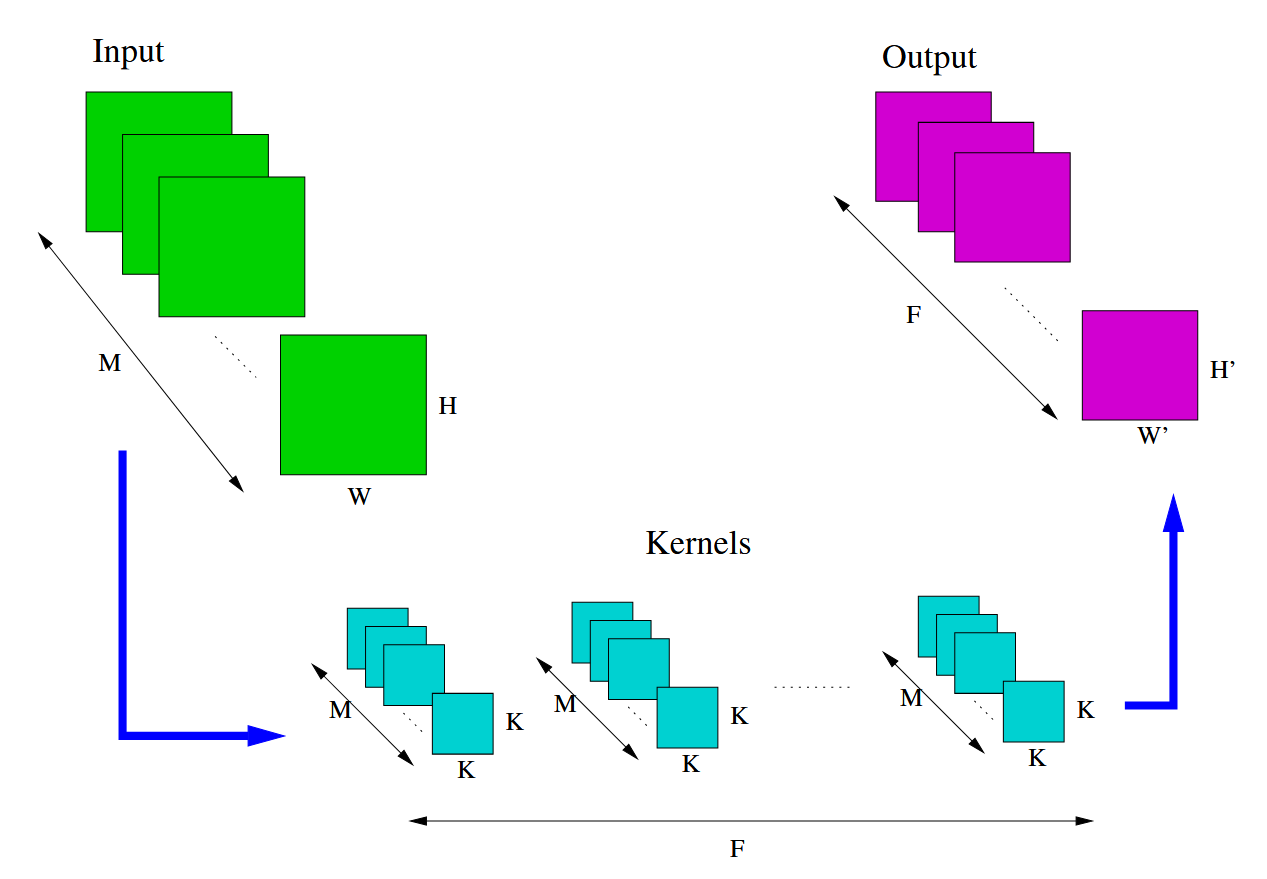
\includegraphics{images/10/convolutionalBlocks.png}
   \caption{Connection between convolutional blocks: each input map has its own set of
filters, but output maps are derived from the related filters}
   \label{fig:10/convolutionalBlocks}
\end{figure}

\begin{itemize}
	\item Input (verde):\\
Sono rappresentate $M$ mappe di input (ad esempio, i canali di un'immagine RGB hanno $M=3$). Ogni mappa ha dimensioni $H \times W$.
	\item Kernels (azzurro):\\
Ogni filtro (kernel) convoluzionale ha dimensioni $K \times K$ e viene applicato a tutte le $M$ mappe di input.
Ci sono $F$ filtri diversi, ognuno dei quali genera una mappa di output.
Ogni filtro è quindi un tensore di dimensioni $M \times K \times K$.
	\item Output (viola):\\
L'applicazione dei $F$ filtri produce $F$ mappe di output, ciascuna di dimensioni $H' \times W'$ (dove $H'$ e $W'$ dipendono da padding e stride).
\end{itemize}


Ogni filtro convoluzionale ``scorre'' su tutte le mappe di input, combinando le informazioni tramite prodotti scalari.
Ogni filtro produce una mappa di output.
Tutte le mappe di output vengono raccolte e formano l'output del blocco convoluzionale.
\nl

\ul{In sintesi}:\\
L'immagine mostra come, partendo da $M$ mappe di input, tramite $F$ filtri convoluzionali (ognuno con profondità $M$), si ottengono $F$ mappe di output. Questo è il cuore del funzionamento di un blocco convoluzionale nelle CNN.
\nl
\nl


Last convolutional block output is a set of 2D maps (matrices)
Classification block expects 1D input (vector)
Flattening operation is needed to pass from 2D to 1D
Flattening size is
\[\frac{F}{S^2p^2} (H + 2P - (K - 1))(W + 2P - (K-1))\]
\note{$(H, W)$ size of input maps for last conv block, with $F$ filters of size $K$ , padding $P$, stride $S$, pooling size $p$}

Classification block:
\begin{itemize}
	\item Input layer: size of flattening
	\item Output layer: size of class number, softmax activation
	\item Hidden layers: size usually reducing
\end{itemize}

Much more parameters in this block than in convolutional blocks

Additional operations: dropout, batch normalisation

\section{CNN Architectures}
Specific tasks require specific structures of convolutional and
non-convolutional blocks.
Many different CNN architectures have been developed over the years, each with specific strengths and applications. The following are some of the most influential CNN architectures in the field:

% \subsection{LeNet-5}
% One of the earliest CNN architectures, proposed by Yann LeCun in 1998. It was designed for handwritten digit recognition and consisted of two convolutional layers followed by three fully connected layers.

% \subsection{AlexNet}
% Winner of the 2012 ImageNet competition, AlexNet significantly outperformed previous approaches and brought CNNs into the mainstream. Key innovations included using ReLU activations, dropout for regularization, and data augmentation.

\subsection{VGGNet}
\begin{figure}[htbp]
   \centering
   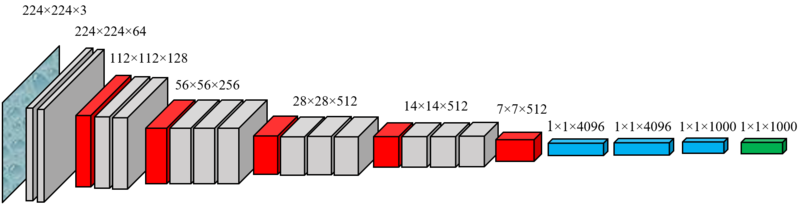
\includegraphics{images/10/vgg.png}
   \caption{VGGNet}
   \label{fig:10/vgg}
\end{figure}
Introduced by the Visual Geometry Group at Oxford, VGG networks (particularly VGG-16 and VGG-19) feature a simple, uniform architecture with small (3×3) convolutional filters stacked deeply. They demonstrated that depth is crucial for performance.

% \subsection{GoogLeNet/Inception}
% This architecture introduced the "Inception module" that processes the input in parallel through different filter sizes and then concatenates the results. This allows the network to capture features at different scales simultaneously while being computationally efficient.

\subsection{ResNet}

\begin{figure}[htbp]
   \centering
   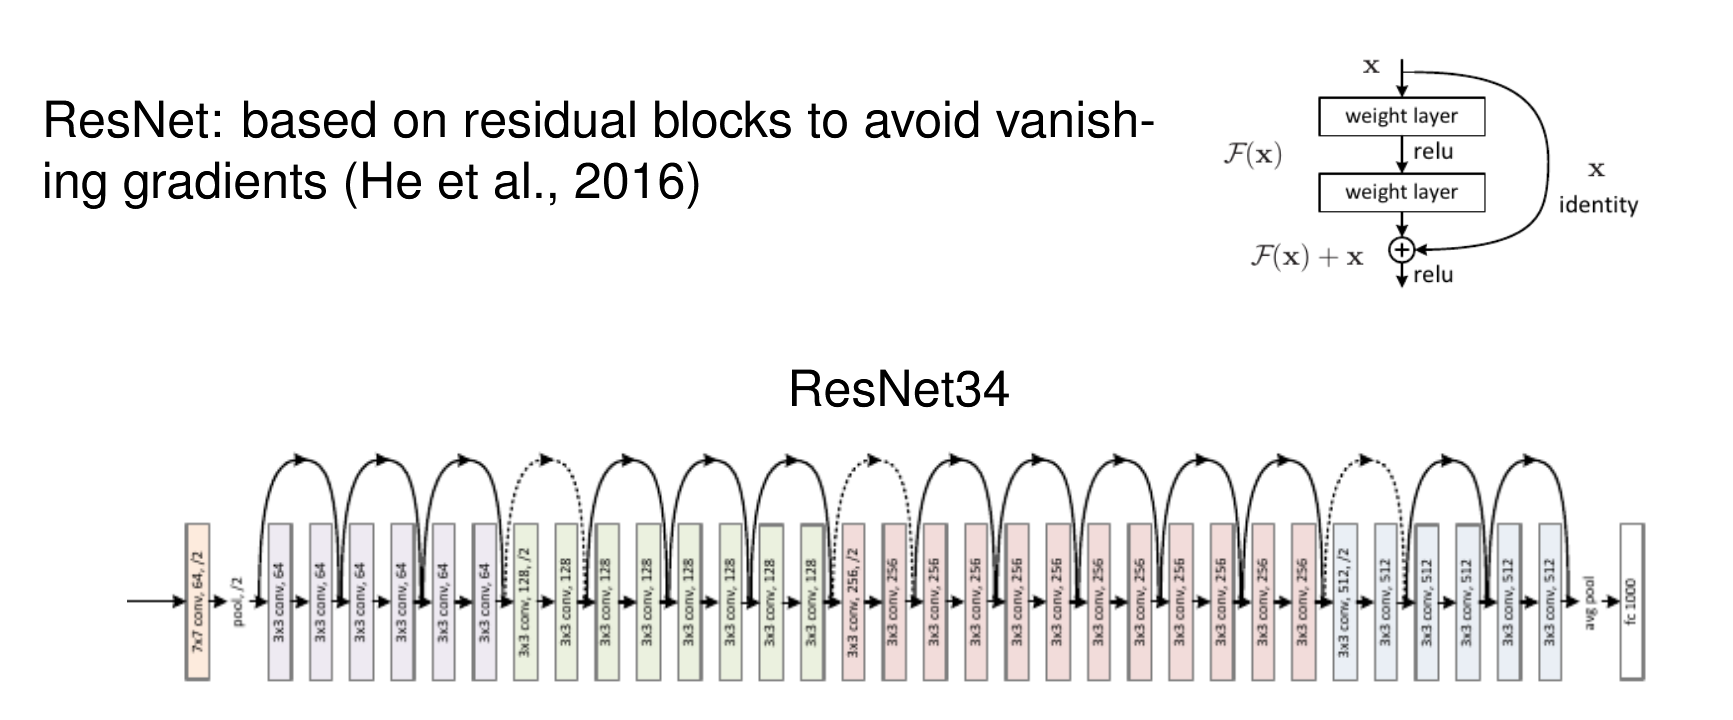
\includegraphics{images/10/resnet.png}
   \caption{ResNet}
   \label{fig:10/resnet}
\end{figure}
Residual Networks address the degradation problem in very deep networks through skip connections or "residual blocks" that allow gradients to flow through the network more easily. ResNet made it possible to train networks with hundreds or even thousands of layers.

% \subsection{MobileNet}
% Designed for mobile and embedded devices, MobileNet uses depthwise separable convolutions to create lightweight models with reduced parameters while maintaining reasonable accuracy.

% \subsection{EfficientNet}
% Proposed a principled method for scaling networks in terms of depth, width, and resolution to achieve better performance with fewer parameters. Uses compound scaling to balance all dimensions of the network.

\subsection{Detection Architectures}
\begin{figure}[htbp]
   \centering
   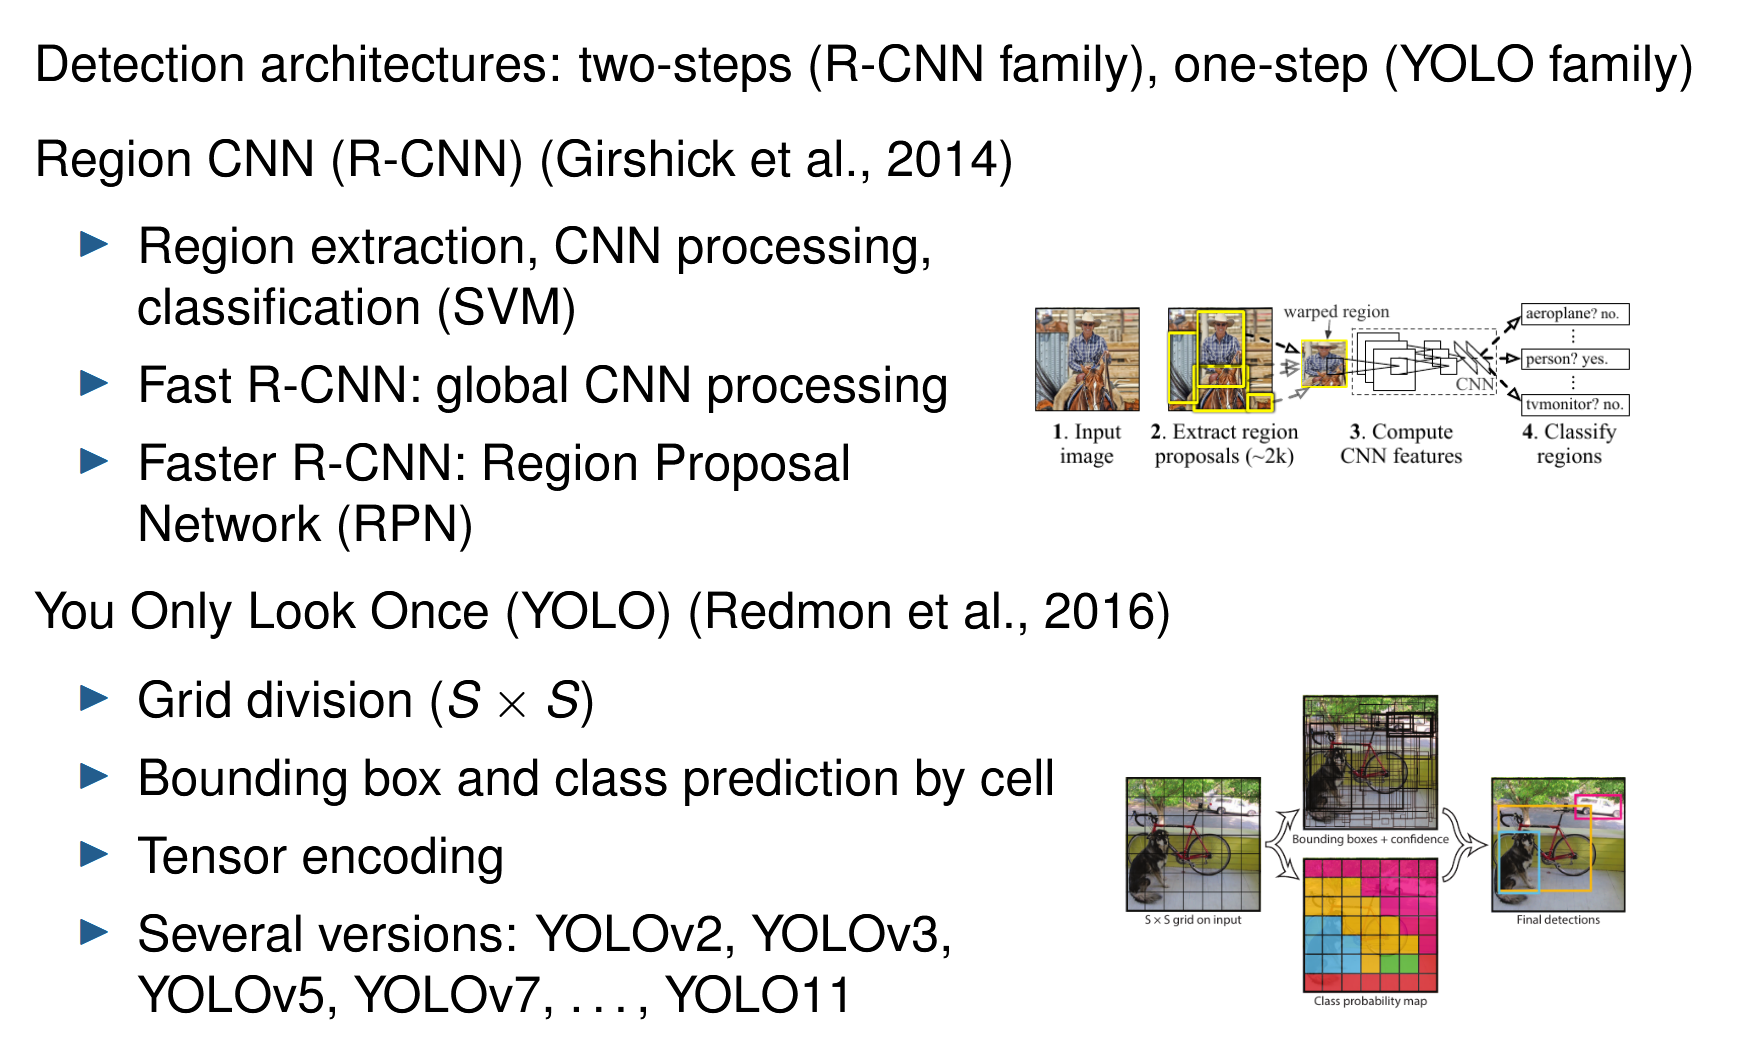
\includegraphics{images/10/detectionArch.png }
   \caption{R-CNN vs YOLO}
   \label{fig:10/detectionArch}
\end{figure}

\subsubsection{R-CNN}
Region-based Convolutional Neural Networks (R-CNN) is a family of models designed for object detection. The original R-CNN proposed a two-stage approach: first, it generates region proposals using selective search, and then it classifies these regions using a CNN. This method significantly improved object detection performance compared to traditional methods.
R-CNN has evolved into several variants, including Fast R-CNN and Faster R-CNN, which improve speed and accuracy by integrating region proposal networks (RPNs) directly into the architecture.

\subsubsection{YOLO}

You Only Look Once (YOLO) is a real-time object detection system that treats object detection as a single regression problem. Instead of generating region proposals, YOLO divides the image into a grid and predicts bounding boxes and class probabilities directly from the entire image in one pass. This approach allows for faster inference times compared to R-CNN-based methods, making YOLO suitable for real-time applications.
YOLO has undergone several iterations, with improvements in accuracy and speed. The latest versions, such as YOLOv4 and YOLOv5, have introduced various enhancements, including better backbone networks, data augmentation techniques, and advanced loss functions.

\subsection{Segmentation Architectures}

\begin{figure}[htbp]
   \centering
   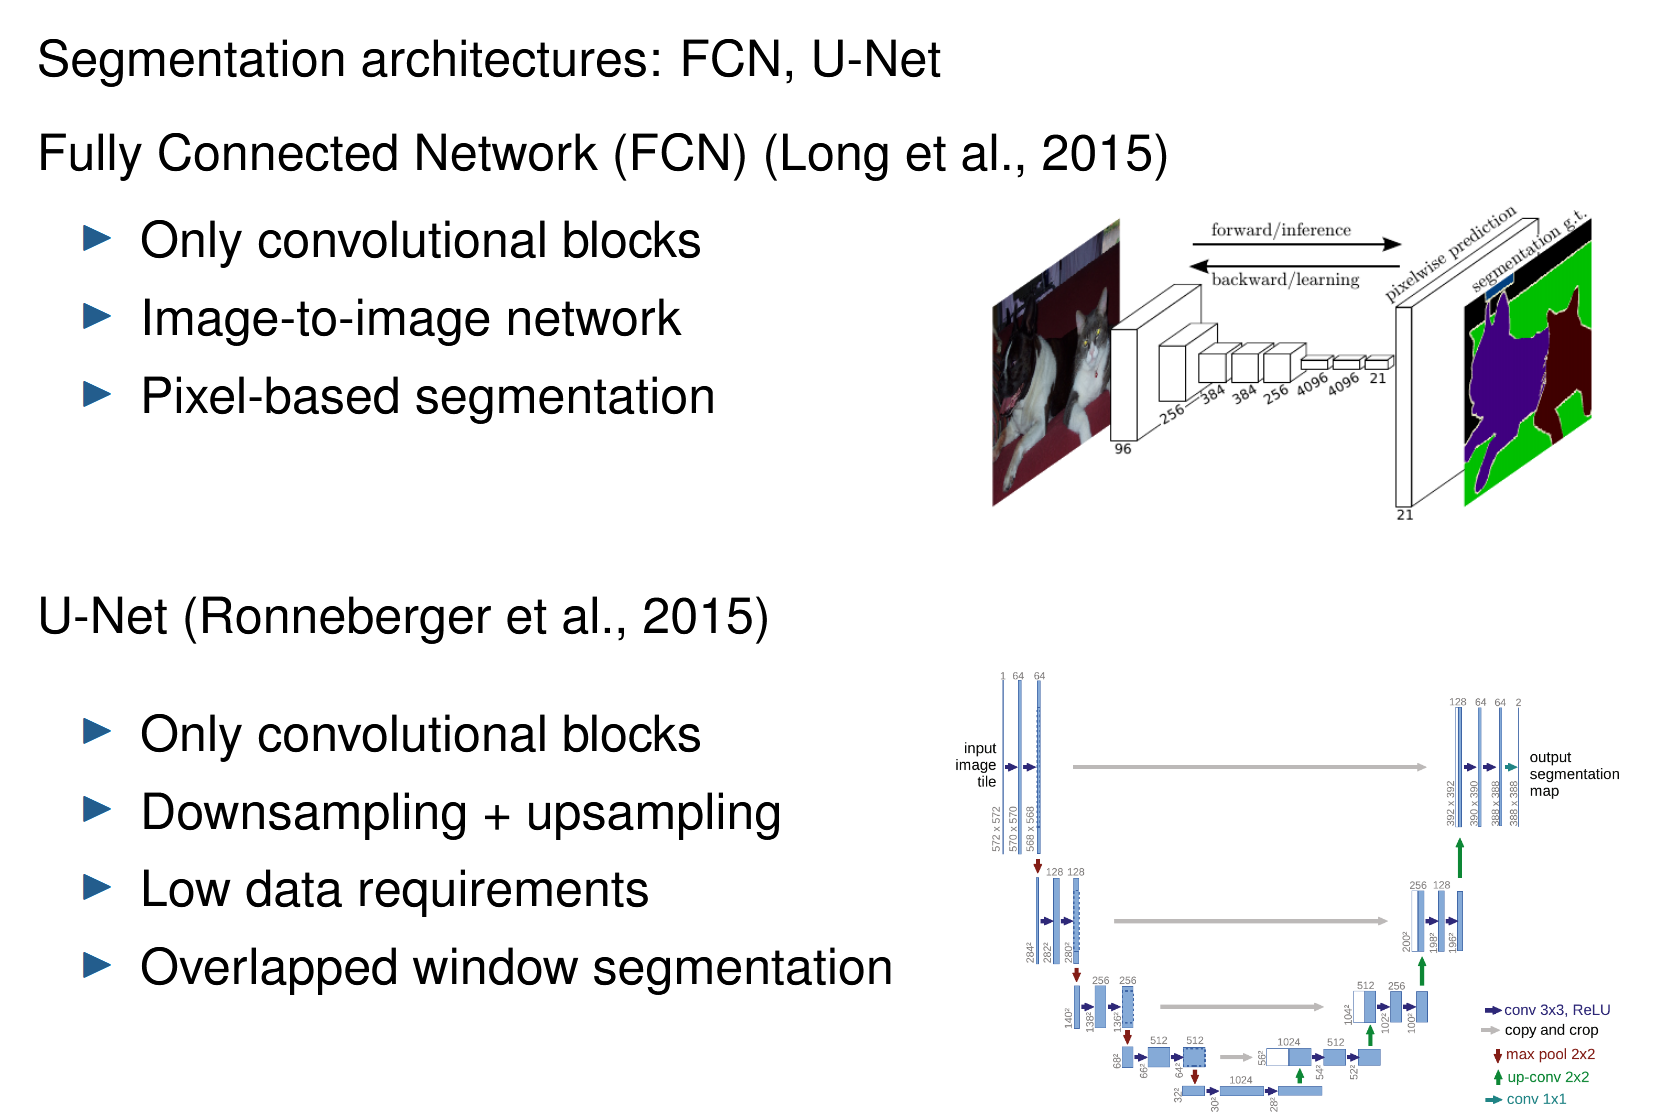
\includegraphics{images/10/segmentationArch.png}
   \caption{Segmentation architectures}
   \label{fig:10/segmentationArch}
\end{figure}
\subsubsection{FCN}

Fully Convolutional Networks (FCNs) are a type of CNN designed for semantic segmentation tasks. Unlike traditional CNNs that output a single label for the entire image, FCNs produce a pixel-wise classification map. This is achieved by replacing fully connected layers with convolutional layers, allowing the network to maintain spatial information throughout the process.
FCNs are trained end-to-end, meaning that the entire network is optimized simultaneously for the segmentation task. They can be used for various applications, including image segmentation, object detection, and scene understanding.
FCNs are built upon standard CNN architectures, but they differ in the following ways:
\begin{itemize}
   \item \textbf{No fully connected layers}: FCNs replace the fully connected layers with convolutional layers, allowing the network to produce output maps of the same spatial dimensions as the input image.
   \item \textbf{Upsampling layers}: FCNs use upsampling (or deconvolution) layers to increase the spatial resolution of the output maps, enabling pixel-wise classification.
   \item \textbf{Skip connections}: FCNs often incorporate skip connections from earlier layers to later layers, allowing the network to combine low-level features with high-level features for better segmentation results.
\end{itemize}

\subsubsection{U-Net}

U-Net is a specialized architecture for semantic segmentation, particularly in biomedical image analysis. It consists of an encoder-decoder structure with skip connections that allow the network to combine low-level features from the encoder with high-level features from the decoder. This helps in preserving spatial information and improving segmentation accuracy.
U-Net is particularly effective for tasks where the amount of training data is limited, as it can learn to produce accurate segmentations even with small datasets. It has been widely adopted in medical imaging, satellite imagery analysis, and other applications requiring precise pixel-wise classification.

\subsection{Transformer Architectures}

\subsubsection{Vision Transformer (ViT)}

Vision Transformer (ViT) is a novel architecture that applies the transformer model, originally designed for natural language processing, to image classification tasks. Instead of using convolutional layers, ViT treats an image as a sequence of patches and processes them using self-attention mechanisms. This allows the model to capture long-range dependencies and relationships between different parts of the image.
ViT has shown competitive performance compared to traditional CNNs, especially when trained on large datasets. It has inspired further research into transformer-based architectures for various computer vision tasks, including object detection and segmentation.
\begin{figure}[htbp]
   \centering
   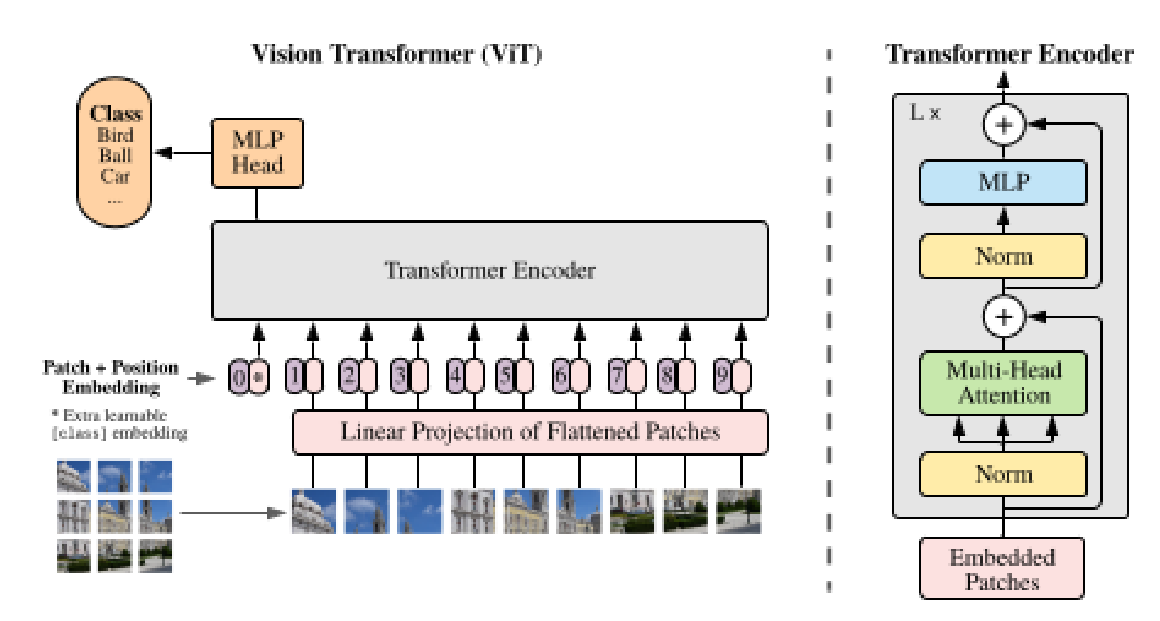
\includegraphics{images/10/vit.png}
   \caption{Vision Transformer}
   \label{fig:10/vit}
\end{figure}

\subsubsection{DeTr (Detection Transformer)}
Detection Transformer (DeTr) is a transformer-based architecture designed for object detection tasks. It combines the strengths of transformers and CNNs to achieve state-of-the-art performance in object detection. DeTr uses a transformer encoder-decoder architecture to process image features and predict bounding boxes and class labels directly.
The key innovation of DeTr is its ability to model relationships between objects in the image using self-attention mechanisms, allowing for better handling of complex scenes and occlusions. This approach eliminates the need for region proposal networks (RPNs) and simplifies the object detection pipeline.
\begin{figure}[htbp]
   \centering
   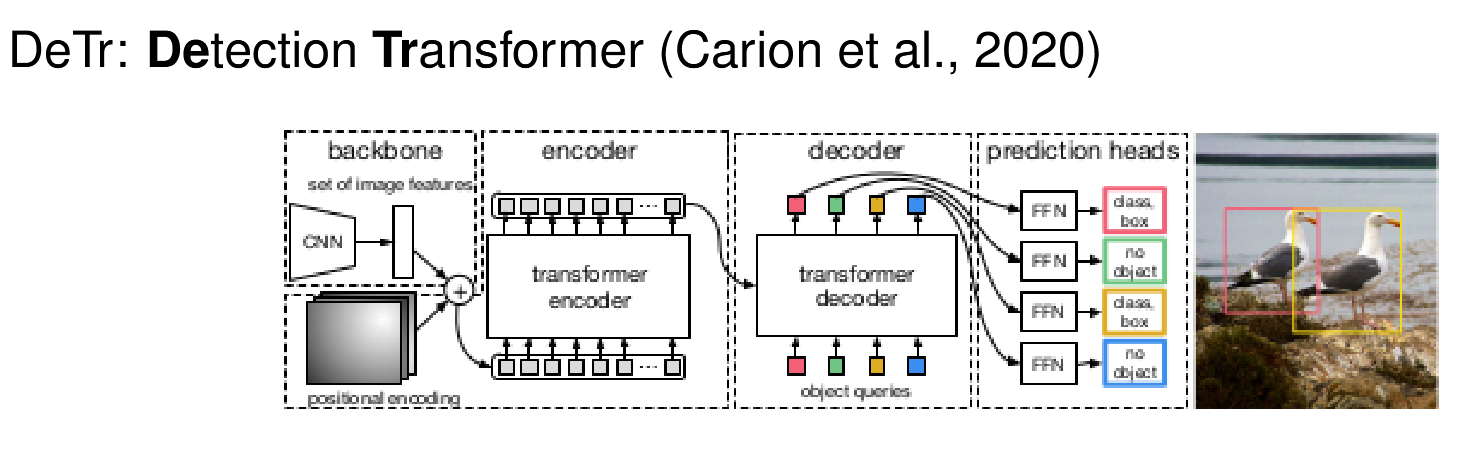
\includegraphics{images/10/detr.png}
   \caption{Detection Transformer}
   \label{fig:10/detr}
\end{figure}
\subsubsection{SeTr (Segmentation Transformer)}
Segmentation Transformer (SeTr) is a transformer-based architecture designed for semantic segmentation tasks. Similar to ViT, SeTr treats images as sequences of patches and applies self-attention mechanisms to capture relationships between different parts of the image. SeTr has shown competitive performance in various segmentation benchmarks, demonstrating the potential of transformers in computer vision tasks.
SeTr uses a transformer encoder-decoder architecture to process image features and predict pixel-wise class labels. The key advantage of SeTr is its ability to model long-range dependencies and relationships between pixels, allowing for better segmentation results in complex scenes.
\begin{figure}[htbp]
   \centering
   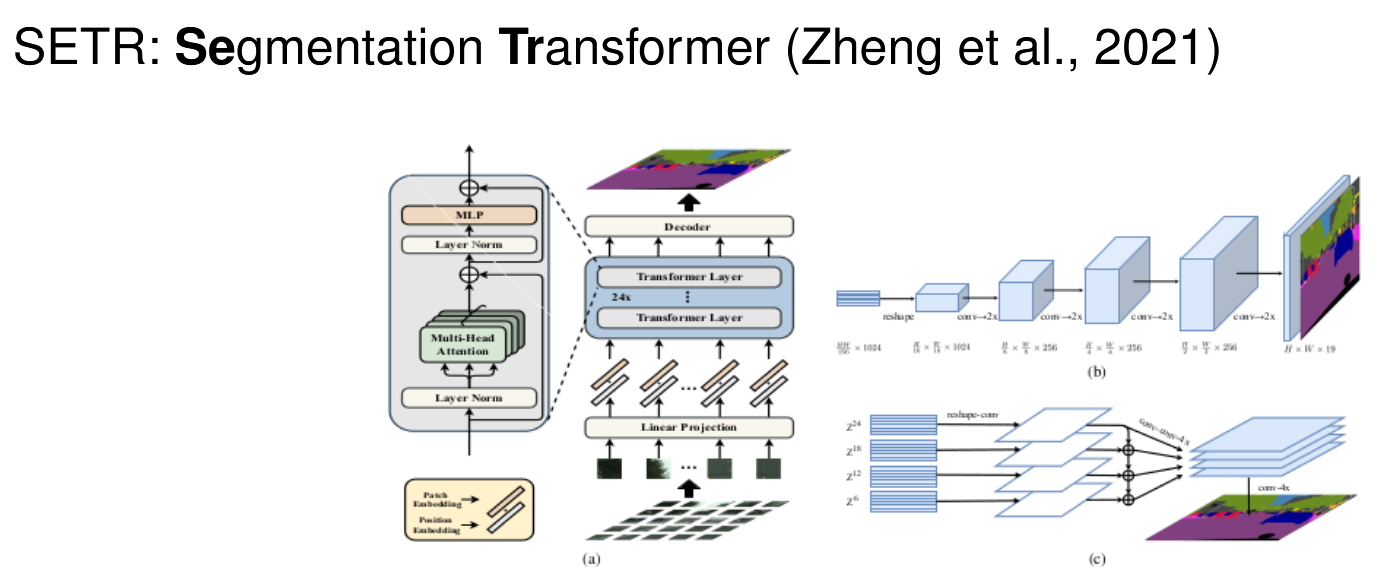
\includegraphics{images/10/setr.png}
   \caption{Segmentation Transformer}
   \label{fig:10/setr}
\end{figure}

\section{Transfer Learning}

Transfer Learning is a technique in deep learning that allows a model trained on one task to be adapted for another related task. This is particularly useful in scenarios where the target task has limited labeled data or when training a model from scratch is computationally expensive.
Transfer learning leverages the knowledge gained from a pre-trained model, which has already learned to extract relevant features from a large dataset. By fine-tuning this model on the target task, we can achieve better performance with less data and training time.
\note{Transfer learning is a powerful technique that allows us to leverage pre-trained models for various tasks, especially when we have limited data or computational resources. It has become a standard practice in deep learning, particularly in computer vision and natural language processing.}

Training from scratch for an image task in DL is difficult
\begin{itemize}
	\item High data requirements
	\item High computational cost (even with specialised hardware)
\end{itemize}
Transfer learning tries to alleviate this problem:
\begin{itemize}
	\item A generic-trained model is taken as init point
	\item The model is changed to fit the task requirements
	\item The model is re-trained with data related task
   \begin{itemize}
   	\item Less data
	   \item Less computational cost
   \end{itemize}
\end{itemize}
In CNN, basically:
\begin{itemize}
	\item Convolutional blocks are kept and classification block is changed
	\item Convolutional weights are frozen in the re-training process
	\item Optional step (fine tuning): unfroze convolutional weights and re-train
\end{itemize}

Transfer learning strategy depends on:
\begin{itemize}
	\item Data availability
	\item Data similarity
	\item Computational resources
\end{itemize}
\nl

\begin{itemize}
	\item High data available and low similarity: train from scratch
	\item High data available and high similarity: freeze a high number of layers
	\item Low data available and low similarity: freeze a low number of layers
	\item Low data available and high similarity: freeze all convolutional layers
   \item[]In case of low computational resources, freeze as much as possible
\end{itemize}